% Created 2016-02-08 Mon 20:43
\documentclass[11pt]{article}
\usepackage[utf8]{inputenc}
\usepackage[T1]{fontenc}
\usepackage{fixltx2e}
\usepackage{graphicx}
\usepackage{longtable}
\usepackage{float}
\usepackage{wrapfig}
\usepackage{rotating}
\usepackage[normalem]{ulem}
\usepackage{amsmath}
\usepackage{textcomp}
\usepackage{marvosym}
\usepackage{wasysym}
\usepackage{amssymb}
\usepackage{hyperref}
\tolerance=1000
\usepackage{minted}
\author{John Cumming}
\date{\today}
\title{Language for 2016 - Common Lisp}
\hypersetup{
  pdfkeywords={},
  pdfsubject={},
  pdfcreator={Emacs 24.5.1 (Org mode 8.2.10)}}
\begin{document}

\maketitle
\tableofcontents


\section{Introduction}
\label{sec-1}

I have chosen common lisp as my language to learn in more depth for
2016 as I have dabbled with it over the past year or so, along with
clojure, another very good lisp based language.

I chose common lisp as a language as I prefer the syntax over
clojure and because I believe it should be able to produce more
efficient code as well as being able to produce stand alone binary
files without the dependence on the JVM that clojure has.

I have no specific plan as to how this learning will pan out, other
than I intend to dive a bit deeper than I have done in the past.

The tools I use for this learning are SBCL and GNU Emacs with
Slime. This is all running under OS-X El Capitan on a Macbook pro.

The complete source code for this article can be found \href{2016-lisp.lisp}{here} and the
article formatted as PDF \href{2016-lisp.pdf}{here}. The org-mode file used to generate
this web page and the lisp code can be found \href{2016-lisp.org}{here}.

Some books I have on lisp can be found \href{books.org}{here}.

I have inter-dispersed larger examples through the code that
hopefully build on the sections that have preceded.

\section{An Overview of Common Lisp Syntax}
\label{sec-2}

Common lisp has a simple syntax for processing lists delimited by '('
and ')'. The lisp processes a list by applying the the first item in
the list as an operator and the rest as operands. Lists can be
nested:

\begin{minted}[linenos,firstnumber=1]{lisp}
;; Comments can be added using a semi colon
(+
 (* 3 4)
 (+ 2 3))
\end{minted}
This code applies operand '+' to the result of applying operand '*'
to 3 and 4, and the result of applying operand '+' to 2 and 3.

A list can be created as a just list of data, by using the 'quote'
operand or by using a shortcut single quote, the following are both
equivalent:

\begin{minted}[linenos,firstnumber=5]{lisp}
;; The following lines are equivalent
(equal (quote (1 2 3 4))
       '(1 2 3 4))
;; => T
\end{minted}

More details on collections can be found in \texttt{Collections}.

String are, like most languages, delimited with double quotes.

Backslashes are used as escape characters, much like other
languages. However, the use of a vertical bar allows special
characters to be used without escaping:

\begin{minted}[linenos,firstnumber=9]{lisp}
;; The following items in the list are equivalent
(equal 'A\(B\) '|A(B)|)
;; => T
\end{minted}

A hash symbol is a macro symbol, known as the dispatching macro
character. There are many of these, for example:

\begin{minted}[linenos,firstnumber=12]{lisp}
;; #' - function abbreviation
;; #\ - character object
;; ,#+ - read-time conditional
;; #c - complex number
;; #( - vector
\end{minted}

More details can be found in \texttt{Macro Dispatching Characters}.

A back quote can be used to allow a template to be used when
generating code, with a comma used to evaluate a form and an '@'
symbol used to splice a list into the template, for example:

\begin{minted}[linenos,firstnumber=17]{lisp}
(defparameter x '(a b c))
;; x
`(x)
;; => (x)
`(,x)
;; => ((a b c))
`(,@x)
;; => (a b c)
`(x ,x ,@x foo ,(cadr x) bar ,(cdr x) baz ,@(cdr x))
;; => (x (a b c) a b c foo b bar (b c) baz b c)
\end{minted}

This is used extensively when writing macros. For more information
on macros see \hyperref[sec-13]{Macros}.

Colons are used in 2 situations. Firstly it can be used to indicate
the package in which a symbol is defined:

\begin{minted}[linenos,firstnumber=27]{lisp}
;; reset is a symbol in the network package
;; (network:reset)
\end{minted}

Packages are discussed in \hyperref[sec-16]{Packages}.

It can also be used to denote a keyword, which is a symbol that
always evaluates to itself and is constant. For example:

\begin{minted}[linenos,firstnumber=29]{lisp}
(eql ':foo :foo)
;; => T
\end{minted}

Keywords are interned in the package KEYWORD and are automatically
exported from it:

\begin{minted}[linenos,firstnumber=31]{lisp}
(eql keyword:foo :foo)
;; => T
\end{minted}

\section{Example 1 - Sum of Square Errors}
\label{sec-3}

An equation that is used in regression algorithms is the sum of
the square of errors for a given dataset and function being fitted
to the data.

Given a data set of size $m$ with a single input variable $x$ and a
single output value $y$ for each item in the data set
and a function that is an attempt to fit a function to the values:

$$y = f(x)$$

Then an error can be calculated based on the sum of the square of
the individual errors, giving an estimate of how well fitted the
function is to the date:

$$E = \sum_{n=0}^m(f(x_n) - y_n)^2$$

Using lisp, we can write some code that takes a data set, computes
the error based on several functions:

\begin{minted}[linenos,firstnumber=33]{lisp}
;; First declare some data
;;
(defparameter data '((0.1 . 1.1)
                     (0.9 . 3.2)
                     (2.1 . 5.9)
                     (3.2 . 7.2)
                     (3.9 . 9.0)
                     (5.1 . 11.2)))

;; then some equations
;;
(defparameter equation-list
  (list #'(lambda (x) (+ 1 (* 2 x)))
        #'(lambda (x) (+ 1 (* x x)))
        #'(lambda (x) (+ 1 x))))

;; now create a function that applies a function
;; to a set of input data
;;
(defun apply-function (f d)
  (map 'list #'(lambda (x) (funcall f (car x))) d))

;; A function that returns the error as the difference
;; between two values squared
;;
(defun square-error (test-data calc-data)
  (expt (- test-data calc-data) 2))

;; A function that returns the sum of square errors
;; of a collection of data and the results
;;
(defun sum-square-error (f test-data)
  (reduce #'+
          (map 'list
               #'(lambda (test calc)
                   (square-error (cdr test) calc))
               test-data (apply-function f test-data))))

;; Now we can run the sum of square errors across all equations
;;
(map 'list #'(lambda (eq) (sum-square-error eq data))
     equation-list)
\end{minted}
\begin{center}
\begin{tabular}{rrr}
0.7400005 & 320.44208 & 61.350002\\
\end{tabular}
\end{center}

The data is defined as a set of cons cells with the car equal to an x
value and the cdr equal to a y value. This is the test data that will
be used to check the equations. It uses defparameter, but could
equally be defined inline at Line 73.

The equations are defined as a list of lambda functions modeling the
following equations for fitting to the data:

$y=2x+1$

$y=x^2+1$

$y=x+1$

Again, these could have been defined inline at the point of use. 

The apply-function function takes a function as an argument and a
collection of data as an alist and executes the function taking the
car of each item in the alist as the x value to calculate the y value.

The square-error function takes a single test data y value and a
single calculated value and calculates the square of the error.

The sum-square-error function takes a function f and applies the
\texttt{square-error} function to each item in the test data and the
corresponding calculated output as calculated by the function f.

The output is generated by applying the  sum-square-error function to
each equation using the test data.

It can clearly be seen from both the results of the sum of square
errors and the input data that eqn1 is the best fit.

To confirm this we can plot the data:

\begin{center}
\begin{tabular}{rrrrr}
x & data & eqn1 & eqn2 & eqn3\\
\hline
0.1 & 1.1 & 1.3 & 1.01 & 1.1\\
0.9 & 3.2 & 2.8 & 1.81 & 1.9\\
2.1 & 5.9 & 5.2 & 5.41 & 3.1\\
3.2 & 7.2 & 7.4 & 11.24 & 4.2\\
3.9 & 9.0 & 8.8 & 16.21 & 4.9\\
5.1 & 11.2 & 11.2 & 27.01 & 6.1\\
\end{tabular}
\end{center}

using this gnuplot script:

\begin{minted}[]{gnuplot}
set terminal png nocrop enhanced size 400,400
set key left box linestyle -1
set xlabel 'x'
set ylabel 'y'
set title 'equation fit'
plot data u 1:2 w p lw 2 title 'data', \
     data u 1:3 smooth csplines lw 1 title 'eqn1', \
     data u 1:4 smooth csplines lw 1 title 'eqn2', \
     data u 1:5 smooth csplines lw 1 title 'eqn3'
\end{minted}
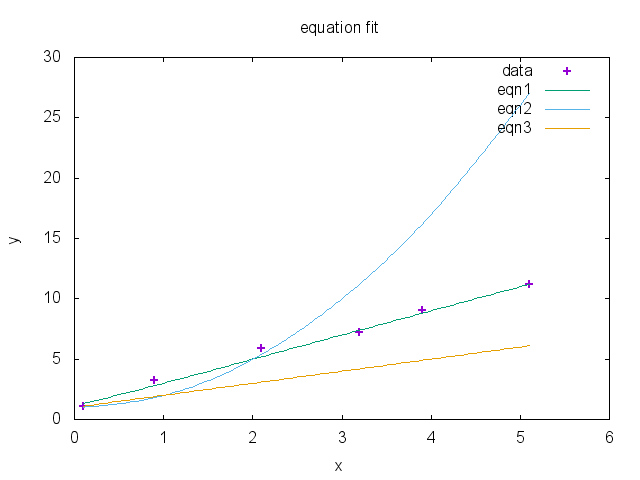
\includegraphics[width=.9\linewidth]{example1-plot.png}

\section{{\bfseries\sffamily NEXT} Core functions}
\label{sec-4}
\begin{itemize}
\item cons

cons is used to construct lists, it puts a new element at the end
of the list, or can be used for creating a pair:
\end{itemize}

\begin{minted}[linenos,firstnumber=75]{lisp}
(cons 1 3)
;; => (1 . 3)
(cons 3 nil)
;; => (3)
(cons 5 '(1 2 3 4))
;; => (5 1 2 3 4)
\end{minted}

\begin{itemize}
\item car

Given a list car retrieves the first item in a list:
\end{itemize}

\begin{minted}[linenos,firstnumber=81]{lisp}
(car '(1 2 3 4))
;; => 1
\end{minted}

\begin{itemize}
\item cdr

Given a list cdr retrieves the remaining list after the first
element
\end{itemize}

\begin{minted}[linenos,firstnumber=83]{lisp}
(cdr '(1 2 3 4))
;; => (2 3 4)
\end{minted}

\begin{itemize}
\item cadr / cddr etc

These can be nested to various levels for example:
\end{itemize}

\begin{minted}[linenos,firstnumber=85]{lisp}
(cadr '(1 2 3 5))
;; => 2
(cddr '(1 2 3 4))
;; => (3 4)
\end{minted}

\begin{itemize}
\item lambda

lambda is used to create a function special form involving a
lambda expression. The expression takes a lambda list and a form
and returns a function:
\end{itemize}

\begin{minted}[linenos,firstnumber=89]{lisp}
(lambda (x) (+ 1 x))
;; => #<FUNCTION (LAMBDA (X)) {10035B665B}>
\end{minted}

\begin{itemize}
\item funcall

Funcall is used to call a function, which can be created with a
lambda.  However it becomes more useful when passing lambda expressions or
functions as arguments (a little convoluted):
\end{itemize}

\begin{minted}[linenos,firstnumber=91]{lisp}
(funcall (lambda (x) (+ 1 x)) 3)
;; => 4

(defun do-something (x a)
  (funcall x a))
(do-something (lambda (x) (+ 1 x)) 2)
;; => 3
\end{minted}

\begin{itemize}
\item function

With the function function we can return a function from a
function! This can be used to create a form of partial functions:
\end{itemize}

\begin{minted}[linenos,firstnumber=98]{lisp}
(defun multiplier (n)
  (function (lambda (x) (* x n))))

(funcall (multiplier 3) 4)
;; => 12

(defun doubler (n)
  (funcall (multiplier 2) n))

(doubler 10)
;; => 20
\end{minted}

\begin{itemize}
\item apply

The apply function is very similar to funcall, except it takes a
list as an argument. This means that it can be used when the
number of arguments is unknown at compile time.
\end{itemize}

\begin{minted}[linenos,firstnumber=109]{lisp}
(apply #'+ 100 '(4 5 6 7))
;; => 122
(defun add-to-ten (&rest args)
  (apply #'+ 10 args))
(add-to-ten 1 2 3 4 5)
;; => 25
\end{minted}

\begin{itemize}
\item read

The read function reads a single s-expression, skipping whitespace
and comments and returns the lisp object denoted by the
s-expression.
\end{itemize}

\begin{minted}[linenos,firstnumber=115]{lisp}
;; given a file code.lisp containing
;;
;; (1 2 3)
;; 456
;; "a string" ; this is a comment
;; ((a b)
;;  (c d))
;;
(defparameter *s* (open "code.lisp"))
;; => *S*
(read *s*)
;; => (1 2 3)
(read *s*)
;; => 456
(read *s*)
;; => "a string"
(read *s*)
;; ((A B) (C D))
(close *s*)
;; => T
\end{minted}

\begin{itemize}
\item eval

The eval function just evaluates a lisp expression. It is used in
combination with read to execute lisp expressions:
\end{itemize}

\begin{minted}[linenos,firstnumber=135]{lisp}
(eval (+ 1 2))
;; => 3
;; given a file code.lisp with a line
;; (+ 1 2)
(defparameter *s* (open "code.lisp"))
(eval (read *s*))
;; => 3
\end{minted}

\begin{itemize}
\item print

The print function prints the representation of a lisp object.
\end{itemize}

\begin{minted}[linenos,firstnumber=142]{lisp}
(print 2)
;; 2
;; => 2
(print (eval (+ 1 2)))
;; 3
;; => 3
\end{minted}

\begin{itemize}
\item cond

The primary conditional statement in lisp is the cond function:
\end{itemize}

\begin{minted}[linenos,firstnumber=148]{lisp}
(defun get-type-name (a)
  (cond ((null a) "null")
        ((atom a) "atom")
        ((listp a) "list")
        (t "unknown")))
(get-type-name nil)
;; => "null"
(get-type-name 1)
;; => "atom"
(get-type-name '(1))
;; => "list"
\end{minted}

\begin{itemize}
\item quote

The quote function is described \texttt{above}.

\item atom

The atom function is outlined \hyperref[sec-5-1]{below}.

\item null

The null function determines if a symbol is nil:
\end{itemize}

\begin{minted}[linenos,firstnumber=159]{lisp}
(null nil)
;; => T
(null 1)
;; => nil
(null '())
;; => T
\end{minted}

\begin{itemize}
\item set setf setq
\item defun var parameter macro etc
\item equality checks
\item declare ?
\end{itemize}

\section{Data Structures}
\label{sec-5}
\subsection{Atoms}
\label{sec-5-1}
Atoms are things that are not cons cells, and can be tested using
the atom predicate:

\begin{minted}[linenos,firstnumber=165]{lisp}
(atom 1)
;; => T
(atom :test)
;; => T
(atom nil)
;; => T
(atom '())
;; => T
\end{minted}

However, they are not things that cannot be broken down any further:

\begin{minted}[linenos,firstnumber=173]{lisp}
(atom "text")
;; => T
(atom #(1 2 3))
;; => T
\end{minted}

Symbols are atoms as well:

\begin{minted}[linenos,firstnumber=177]{lisp}
(defun test-atomicity (x) (atom x))
(atom 'test-atomicity)
;; => T
\end{minted}

And lambda expressions:

\begin{minted}[linenos,firstnumber=180]{lisp}
(atom (lambda (x) (atom x)))
;; => T
\end{minted}

Examples of some things that are not atoms:

\begin{minted}[linenos,firstnumber=182]{lisp}
(atom '(1 . 3))
;; => NIL
(atom '(1 2 3))
;; => NIL
(atom (cdr '(1 2 3)))
;; => NIL
\end{minted}

\subsection{{\bfseries\sffamily NEXT} Sequences}
\label{sec-5-2}
Sequences are ordered lists of elements and can be manipulated by a
variety of standard sequence functions. A sequence is either a
vector or a list. Vectors are one dimensional arrays and Lists are
linked lists made up of cons cells and are discussed \hyperref[sec-5-2-4]{here}.
\subsubsection{Arrays}
\label{sec-5-2-1}
\begin{itemize}
\item simple array
\item bit array
\end{itemize}
\subsubsection{Vectors}
\label{sec-5-2-2}
\begin{itemize}
\item simple vector
\item bit vector
\end{itemize}
\subsubsection{Strings}
\label{sec-5-2-3}
A string is a specialized vector with elements of type
character. All the sequence functions \texttt{below} can be applied to
strings.
\begin{itemize}
\item Manipulating the case of a string
\begin{itemize}
\item string-upcase
\item string-downcase
\item string-capitalize
\item nstring-upcase
\item nstring-downcase
\item nstring-capitalize
\end{itemize}
\item Trimming strings
\begin{itemize}
\item string-trim
\item string-left-trim
\item string-right-trim
\end{itemize}
\item Converting to and from strings
\begin{itemize}
\item intern
\item symbol-name
\item string
\item coerce
\item parse-integer
\item read-from-string
\item write-to-string
\end{itemize}
\item Comparing strings
\begin{itemize}
\item string=
\item string/=
\item string-equal
\item string-not-equal
\item string<
\item string>
\item string<=
\item string>=
\item string-lessp
\item string-greaterp
\item string-not-lessp
\item string-not-greaterp
\end{itemize}
\end{itemize}
\subsubsection{Lists}
\label{sec-5-2-4}
\begin{itemize}
\item Cons Cells
\item Proper List
\item Dotted List
\item Circular List
\end{itemize}
\subsubsection{Manipulating Sequences}
\label{sec-5-2-5}
\begin{itemize}
\item concatenate
\item copy-seq
\item count
\item count-if
\item count-if-not
\item delete
\item delete-duplicates
\item delete-if
\item delete-if-not
\item elt
\item every
\item fill
\item find
\item find-if
\item find-if-not
\item length
\item map
\item mapcar
\item map-into
\item merge
\item mismatch
\item notany
\item notevery
\item nreverse
\item nsubstitute
\item nsubstitute-if
\item nsubstitute-if-not
\item position
\item position-if
\item position-if-not
\item reduce
\item remove
\item remove-duplicates
\item remove-if
\item remove-if-not
\item replace
\item reverse
\item search
\item some
\item sort
\item stable-sort
\item subseq
\item substitute
\item substitute-if
\item substitute-if-not
\end{itemize}
\subsection{Hash Tables}
\label{sec-5-3}
\subsection{Trees}
\label{sec-5-4}
\subsection{Association Lists}
\label{sec-5-5}
\subsection{Property Lists}
\label{sec-5-6}
\subsection{Records}
\label{sec-5-7}
\subsection{Structures}
\label{sec-5-8}
\subsection{Classes}
\label{sec-5-9}
\section{Creating Variables}
\label{sec-6}
\section{Functions}
\label{sec-7}
currying / partial
no side effects
let / flet 
\section{Control Operations}
\label{sec-8}
\section{Error Handling}
\label{sec-9}
\section{Lazyiness}
\label{sec-10}
\section{Streams}
\label{sec-11}
\section{Macro Dispatching Characters}
\label{sec-12}
set-macro-character
symbol macros
\section{Macros}
\label{sec-13}
\section{Multimethods}
\label{sec-14}
\section{CLOS}
\label{sec-15}
\section{Packages}
\label{sec-16}
\section{Standard Libraries}
\label{sec-17}
\section{Important Libraries}
\label{sec-18}
\section{Working with GNU Emacs and Slime}
\label{sec-19}
% Emacs 24.5.1 (Org mode 8.2.10)
\end{document}